\documentclass[12pt]{report}

\usepackage{graphicx}
\graphicspath{ {./images} }

\usepackage{parskip}
\setlength{\parskip}{\baselineskip}
\setlength{\parindent}{0pt}

\title{Jane Goodall Script}
\author{Rayhan \and Odi \and Bagas}

\begin{document}

\maketitle

\centering

\section*{Orientation of Jane Goodall}

Meet Jane Goodall, one of the pioneering English primatologists. Goodall is
well known for her expansive research and dedication in order to save the lives
of chimpanzees around the world.

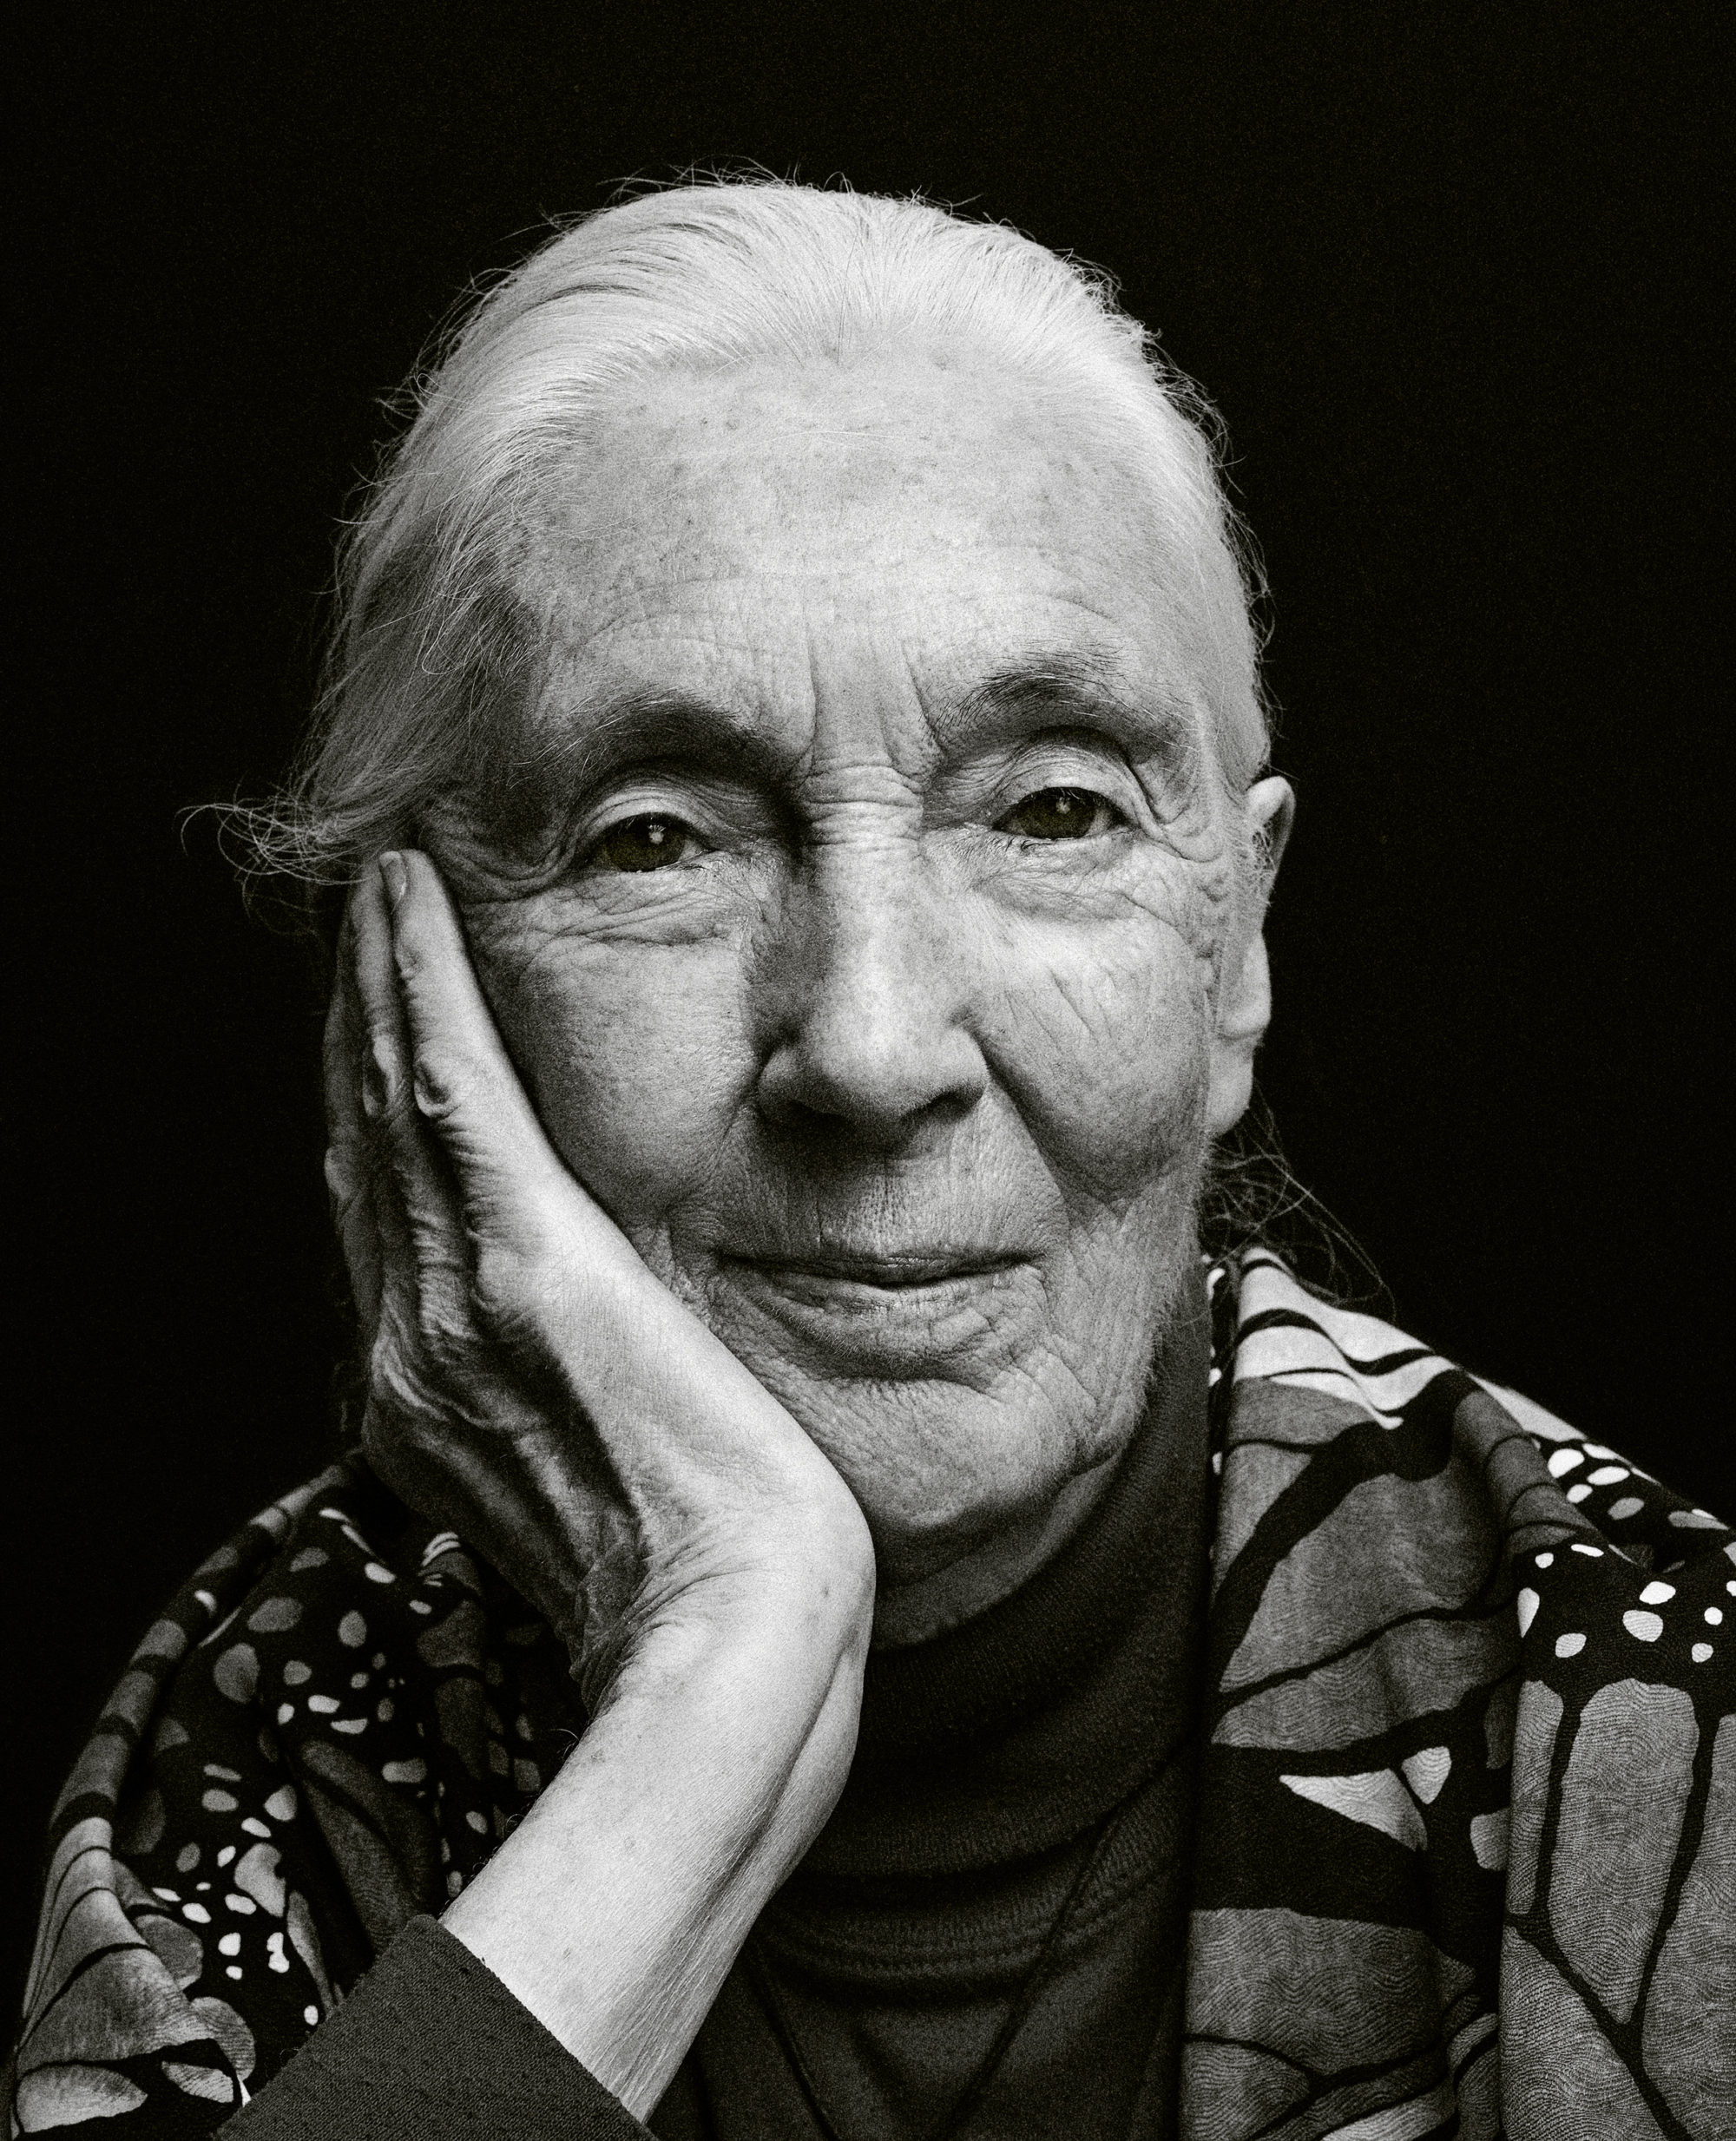
\includegraphics[
    width=7cm,
    height=10cm,
    keepaspectratio
]{jane-goodall-introduction}

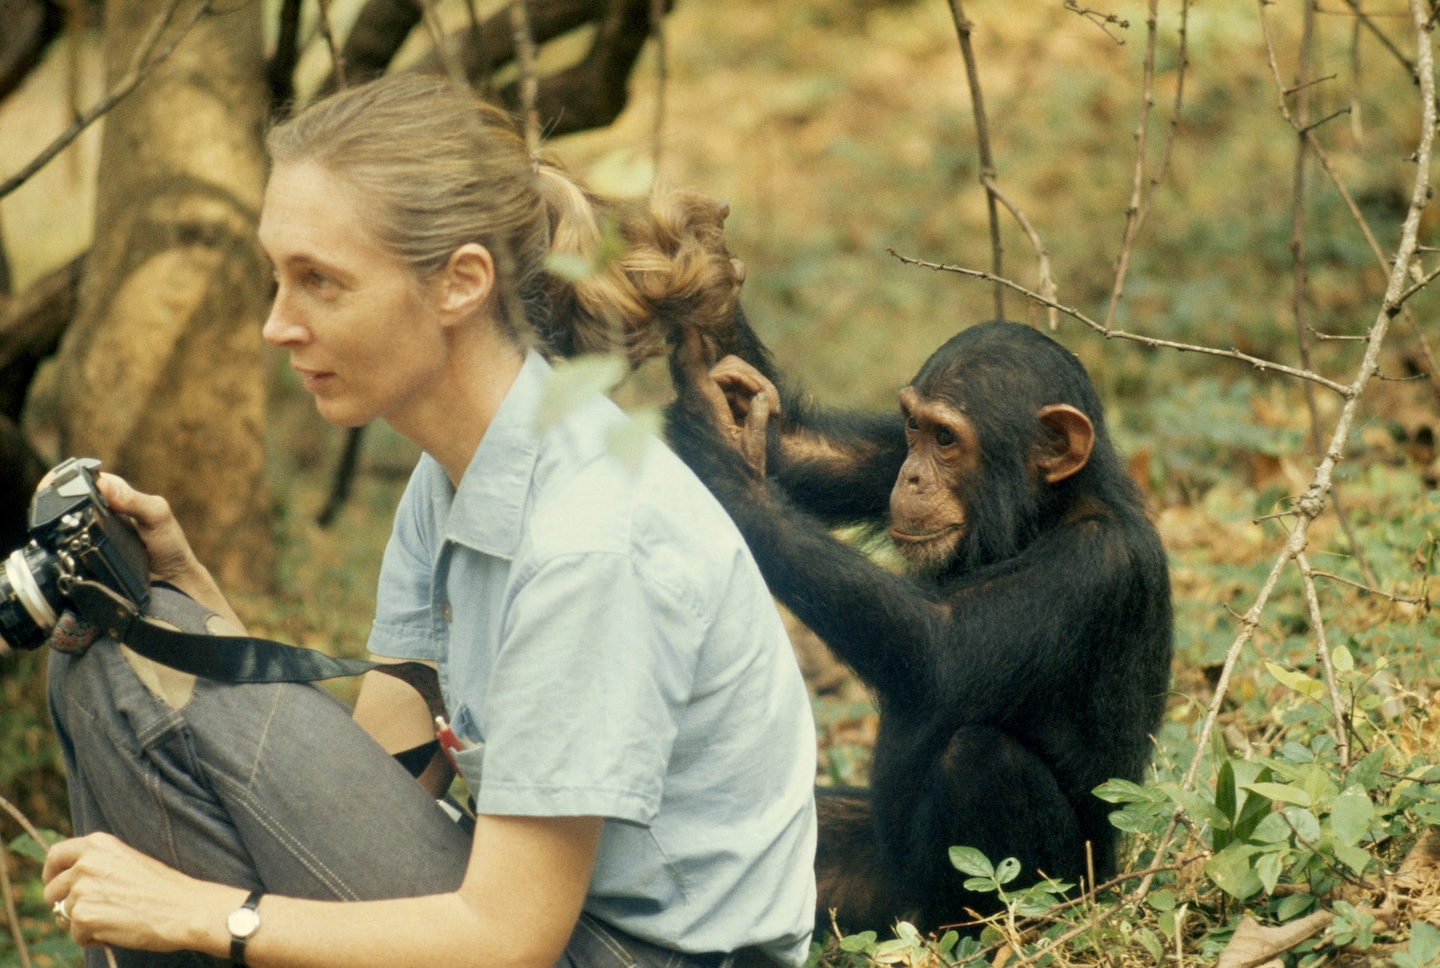
\includegraphics[
    width=10cm,
    height=20cm,
    keepaspectratio
]{jane-goodall-introduction-2}

\pagebreak

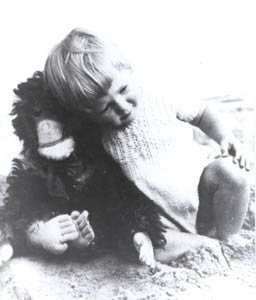
\includegraphics[
    width=6cm,
    height=15cm,
    keepaspectratio
]{jane-goodall-jubilee}

Her sheer passion was all thanks to Jubilee, a chimpanzee doll Goodall acquired
during her first birthday. This was what sparked Goodall's unadulterated
fascination with chimpanzees.

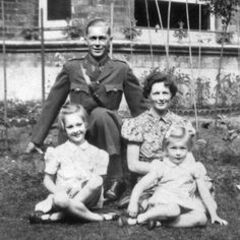
\includegraphics[
    width=6cm,
    height=15cm,
    keepaspectratio
]{jane-goodall-family}

Goodall was the daughter of Margaret Myfanwe Joseph, who worked as a novelist,
and motorsports racer \& businessman Mortimer Morris-Goodall, who was also the
founder of the Aston Martin Owners Club.

\pagebreak

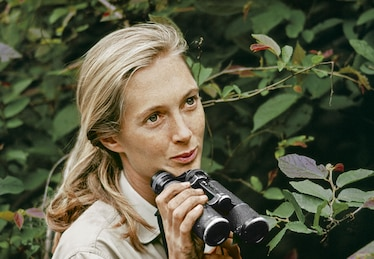
\includegraphics[
    width=8cm,
    height=18cm,
    keepaspectratio
]{jane-goodall-cinematography}

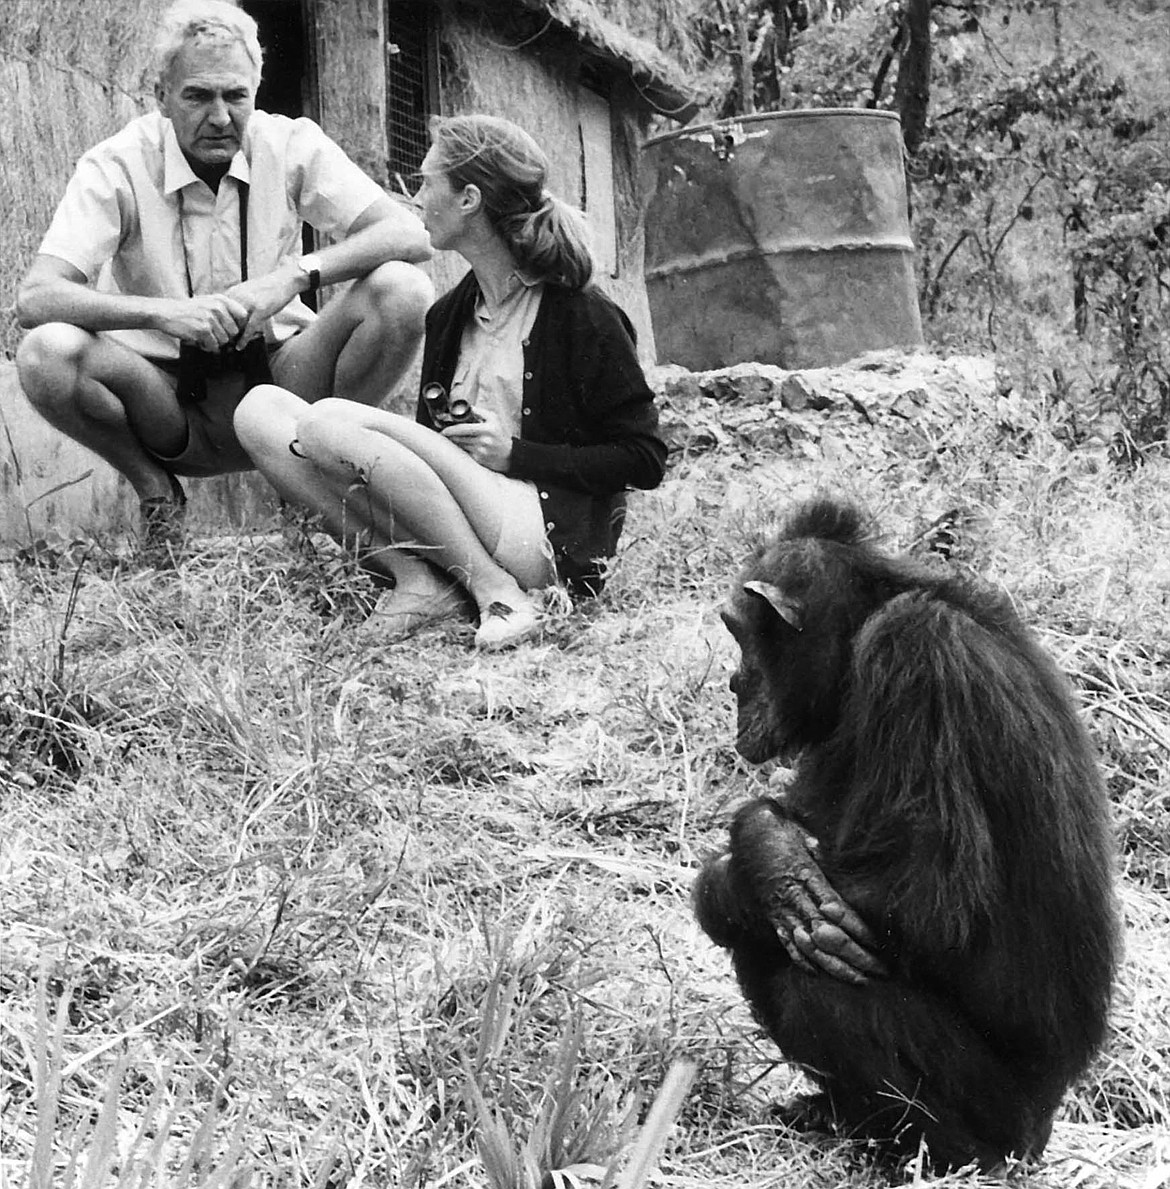
\includegraphics[
    width=8cm,
    height=18cm,
    keepaspectratio
]{jane-goodall-partner}

Aside from an activist, Goodall even worked as a film production assistant and
her own friend's secretary advisor during his research.

\pagebreak

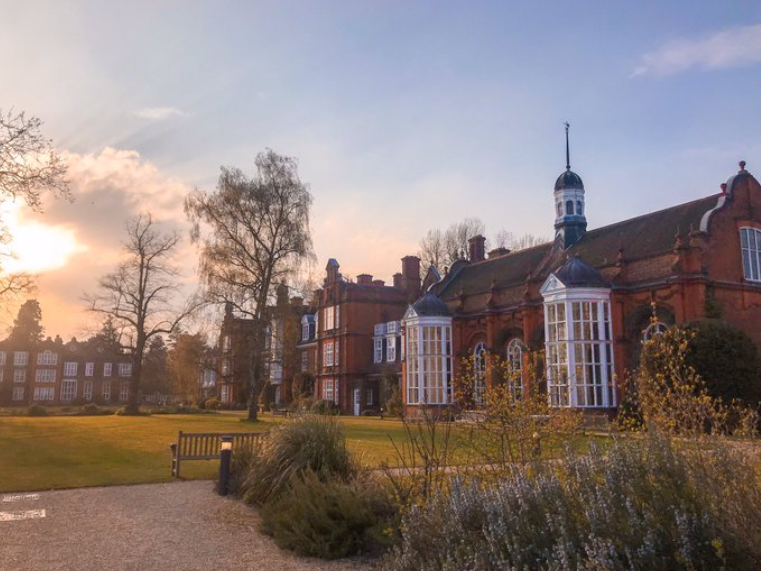
\includegraphics[
    width=10cm,
    height=10cm,
    keepaspectratio
]{newnham-college}

For university, Goodall first went to Newnham College, where she eventually
received her Bachelor of Arts in natural sciences.

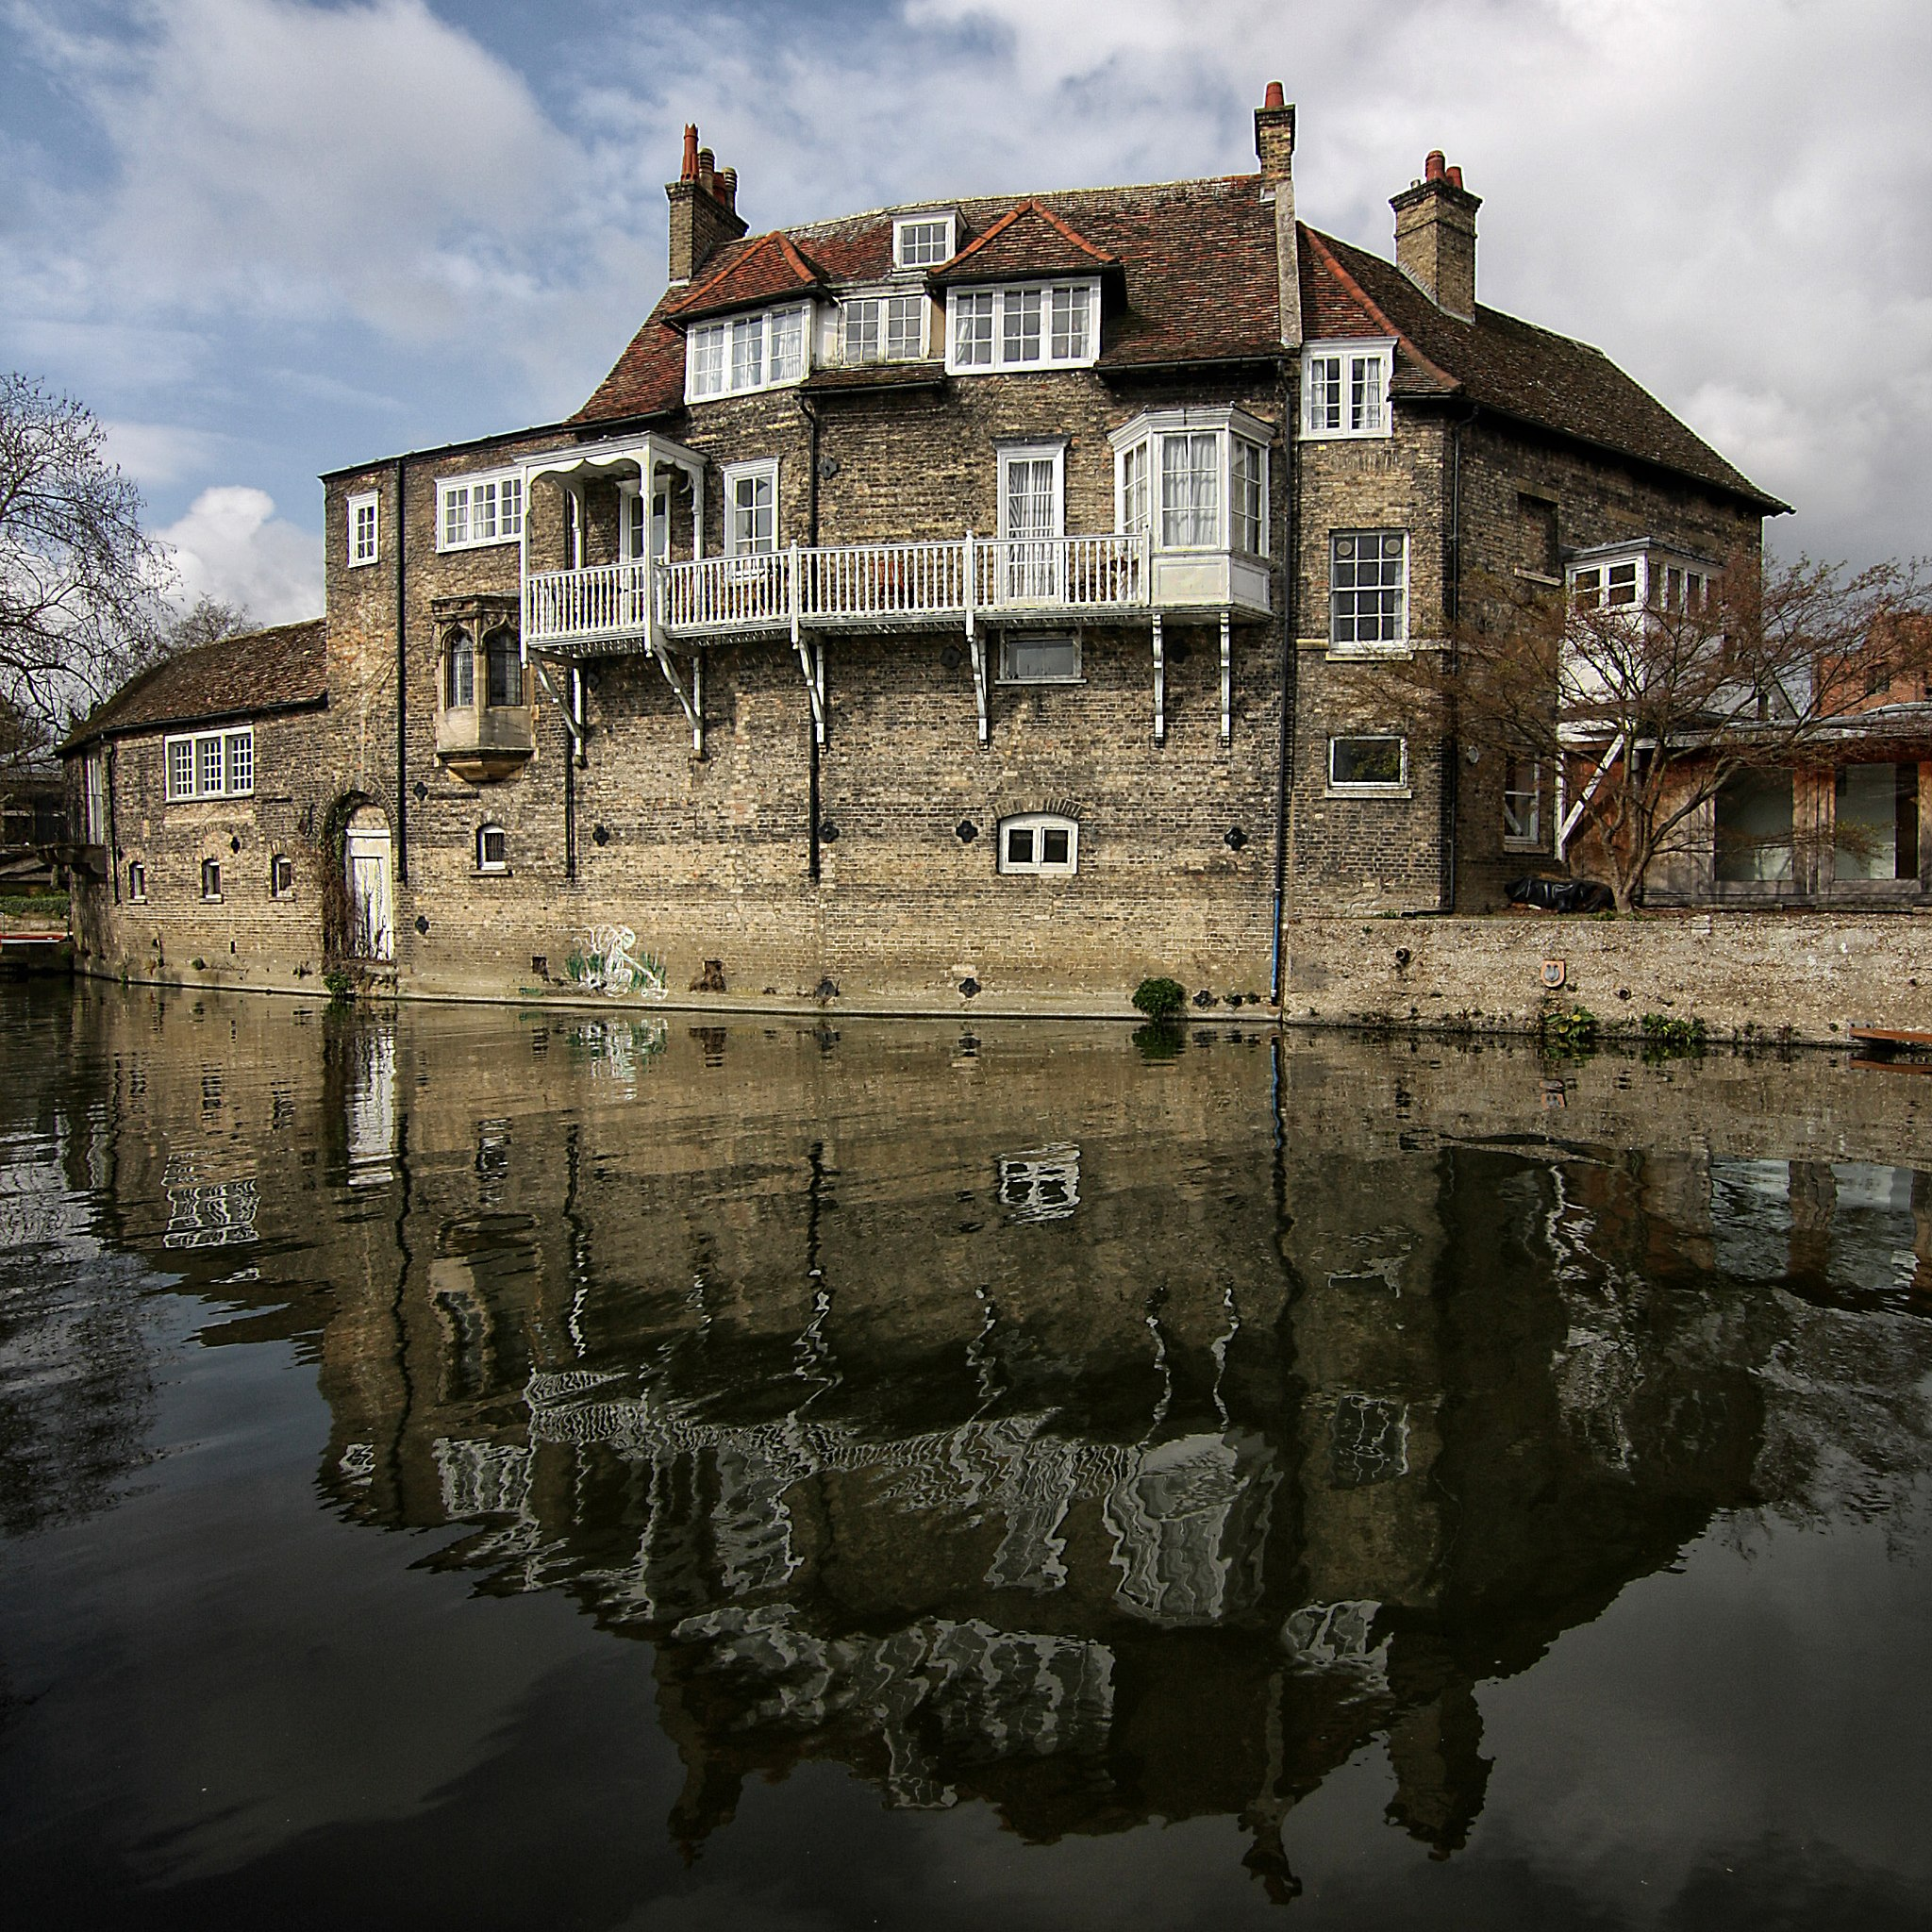
\includegraphics[
    width=8cm,
    height=18cm,
    keepaspectratio
]{darwin-college}

And that is when she attended Darwin College, aiming for a Doctor of Philosophy
in ethology.

\pagebreak

At one point, Goodall was eventually married to Hugo van Lawick from 1964 to
1974 and Derek Bryceson in the year 1975.

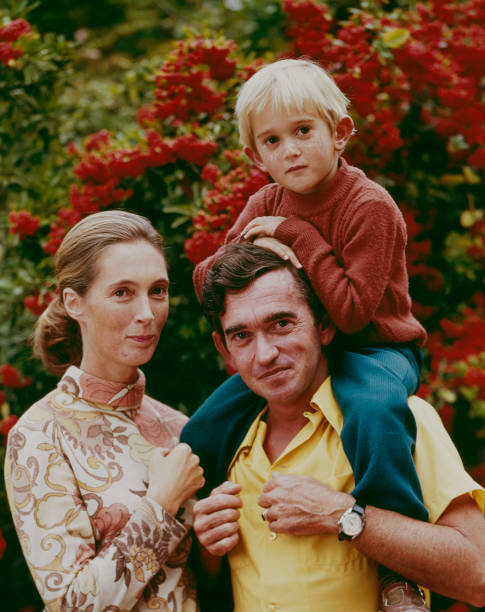
\includegraphics[
    width=7cm,
    height=7cm,
    keepaspectratio
]{jane-goodall-hugo}

Jane Goodall with Hugo Van Lawick

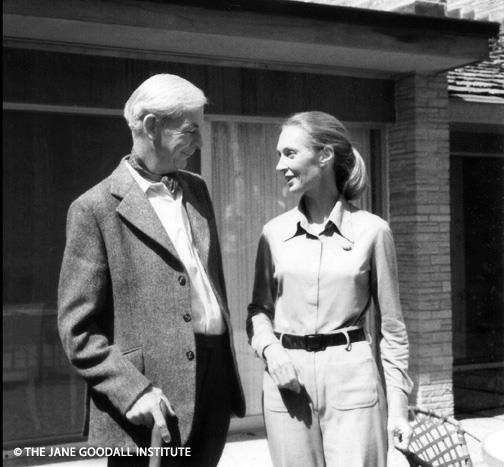
\includegraphics[
    width=8cm,
    height=8cm,
    keepaspectratio
]{jane-goodall-bryceson}

Jane Goodall with Derek Bryceson

\section*{Events of Jane Goodall}

In 1957, Jane Goodall traveled to Kenya to visit his friend family and meet
Louis Leakey, who is a paleontologist and anthropologist.

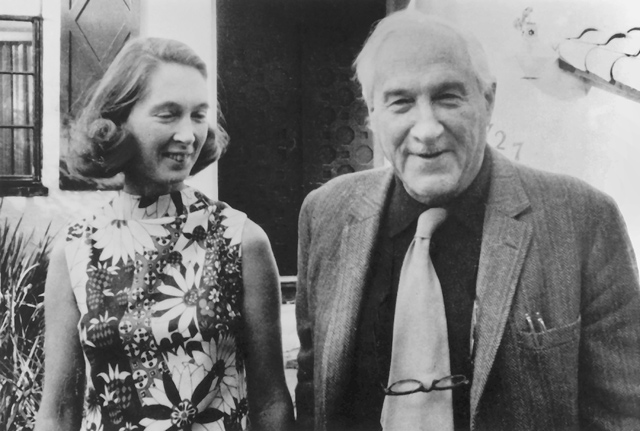
\includegraphics[
    width=10cm,
    height=10cm,
    keepaspectratio
]{jane-goodall-leakey}

During her time in Kenya, she worked as Louis Leaky’s secretary, assisting him
during his research.

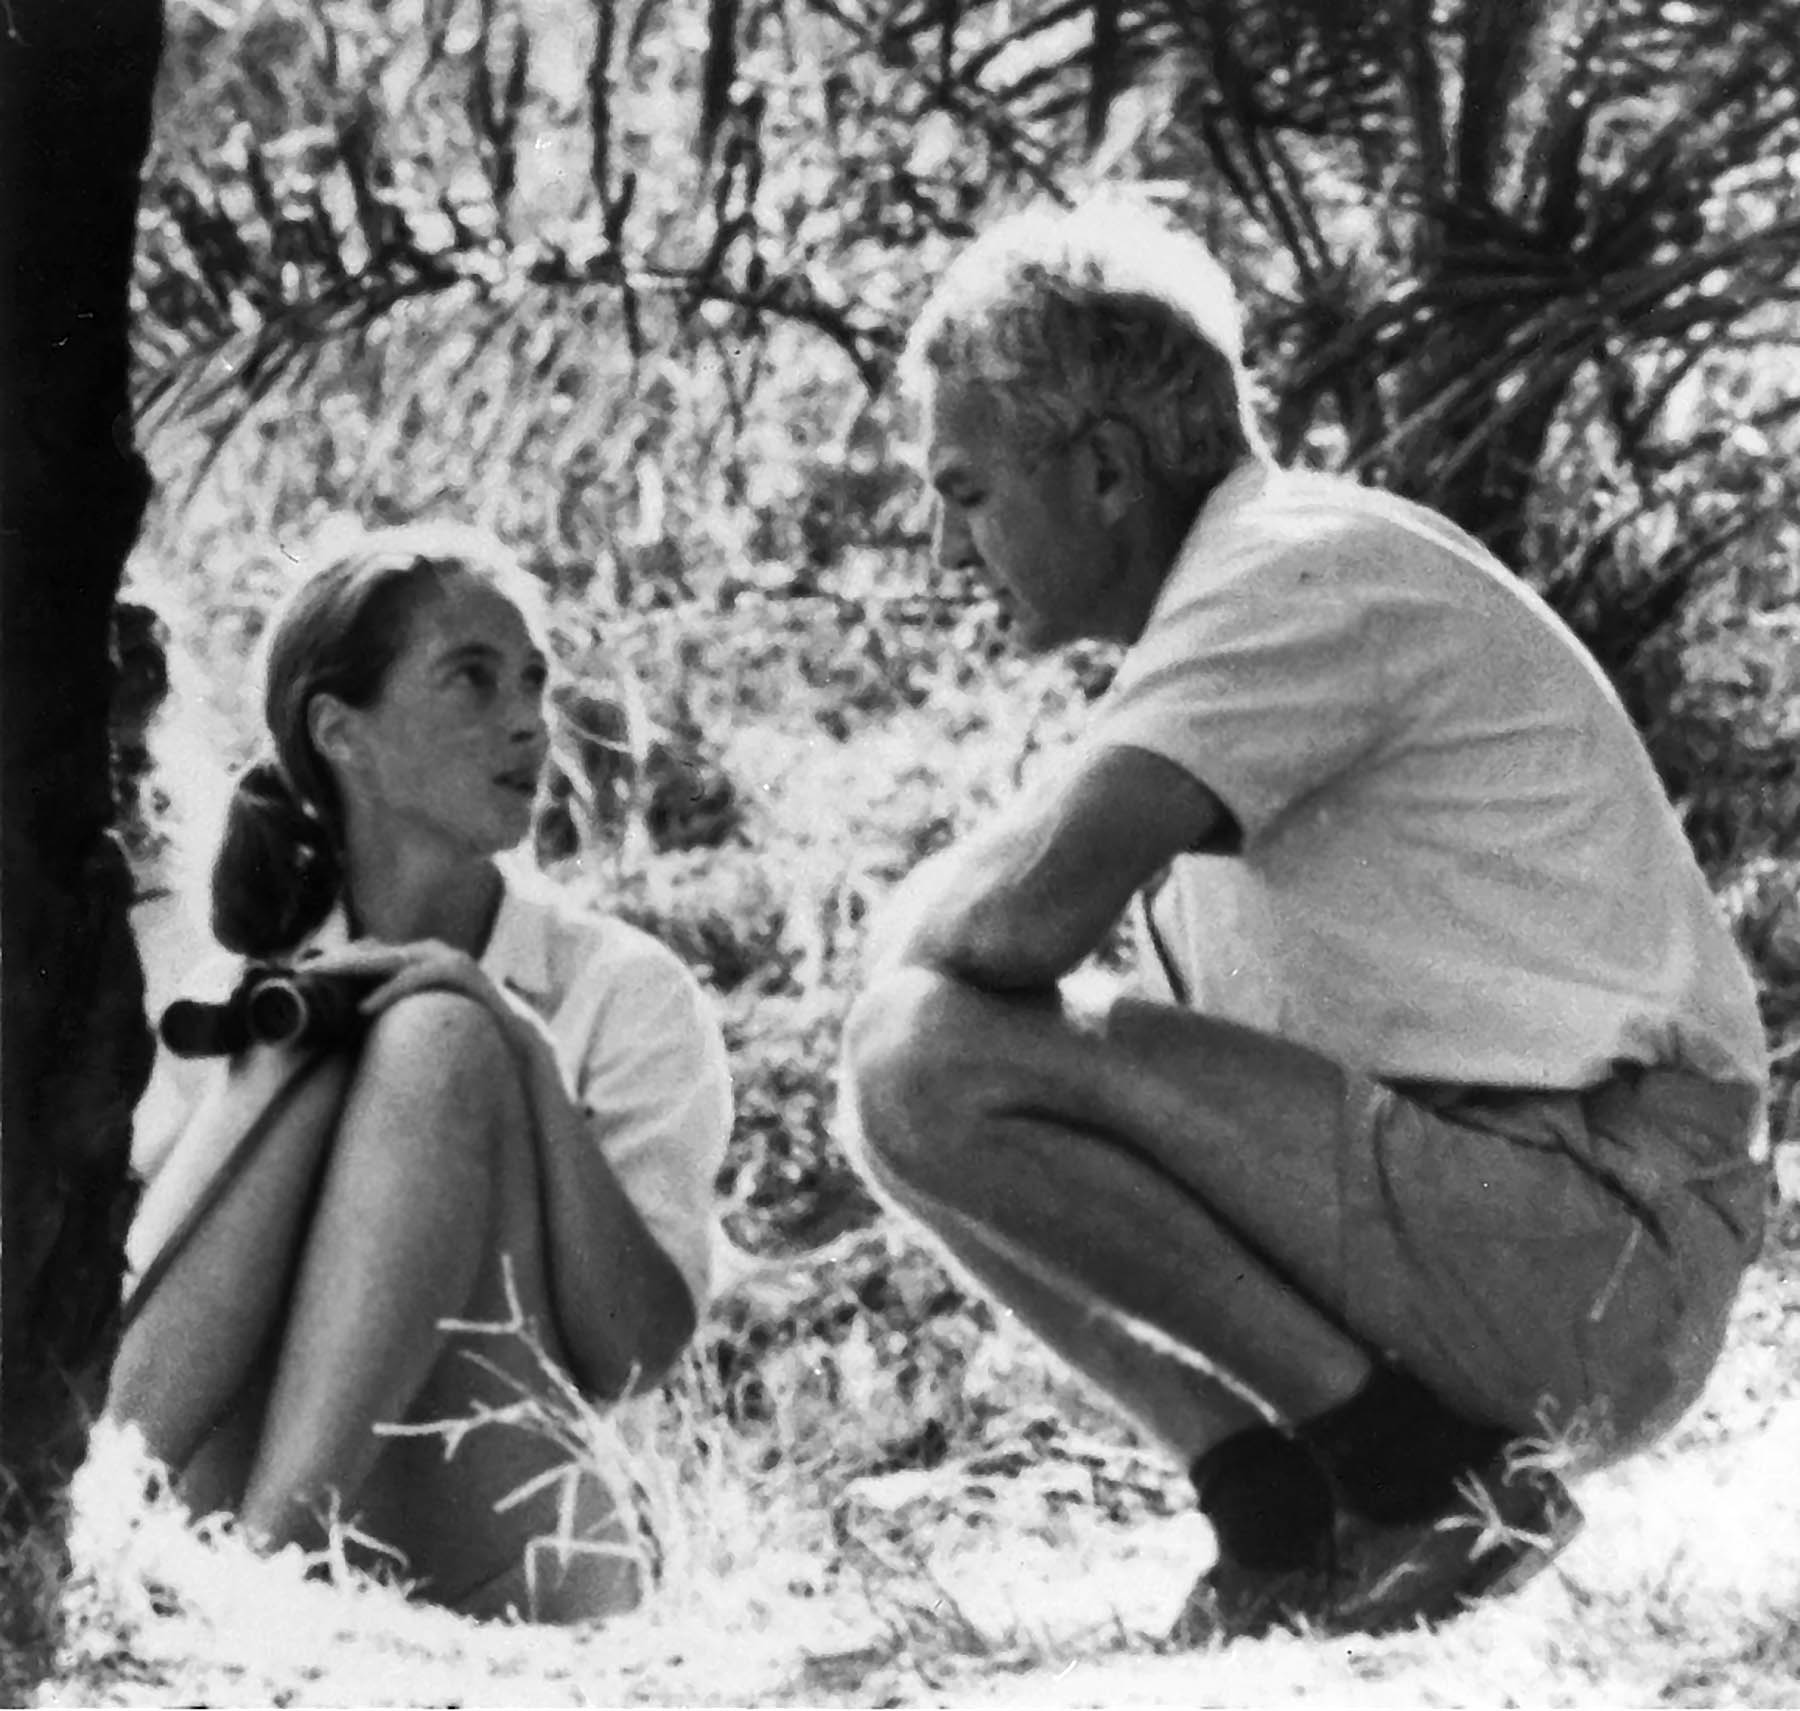
\includegraphics[
    width=8cm,
    height=8cm,
    keepaspectratio
]{jane-goodall-leakey-research}

\pagebreak

3 years later, in 1960, Jane Goodall traveled to Gombe and Tanzania to observe
chimpanzees and their behavior in natural habitat.

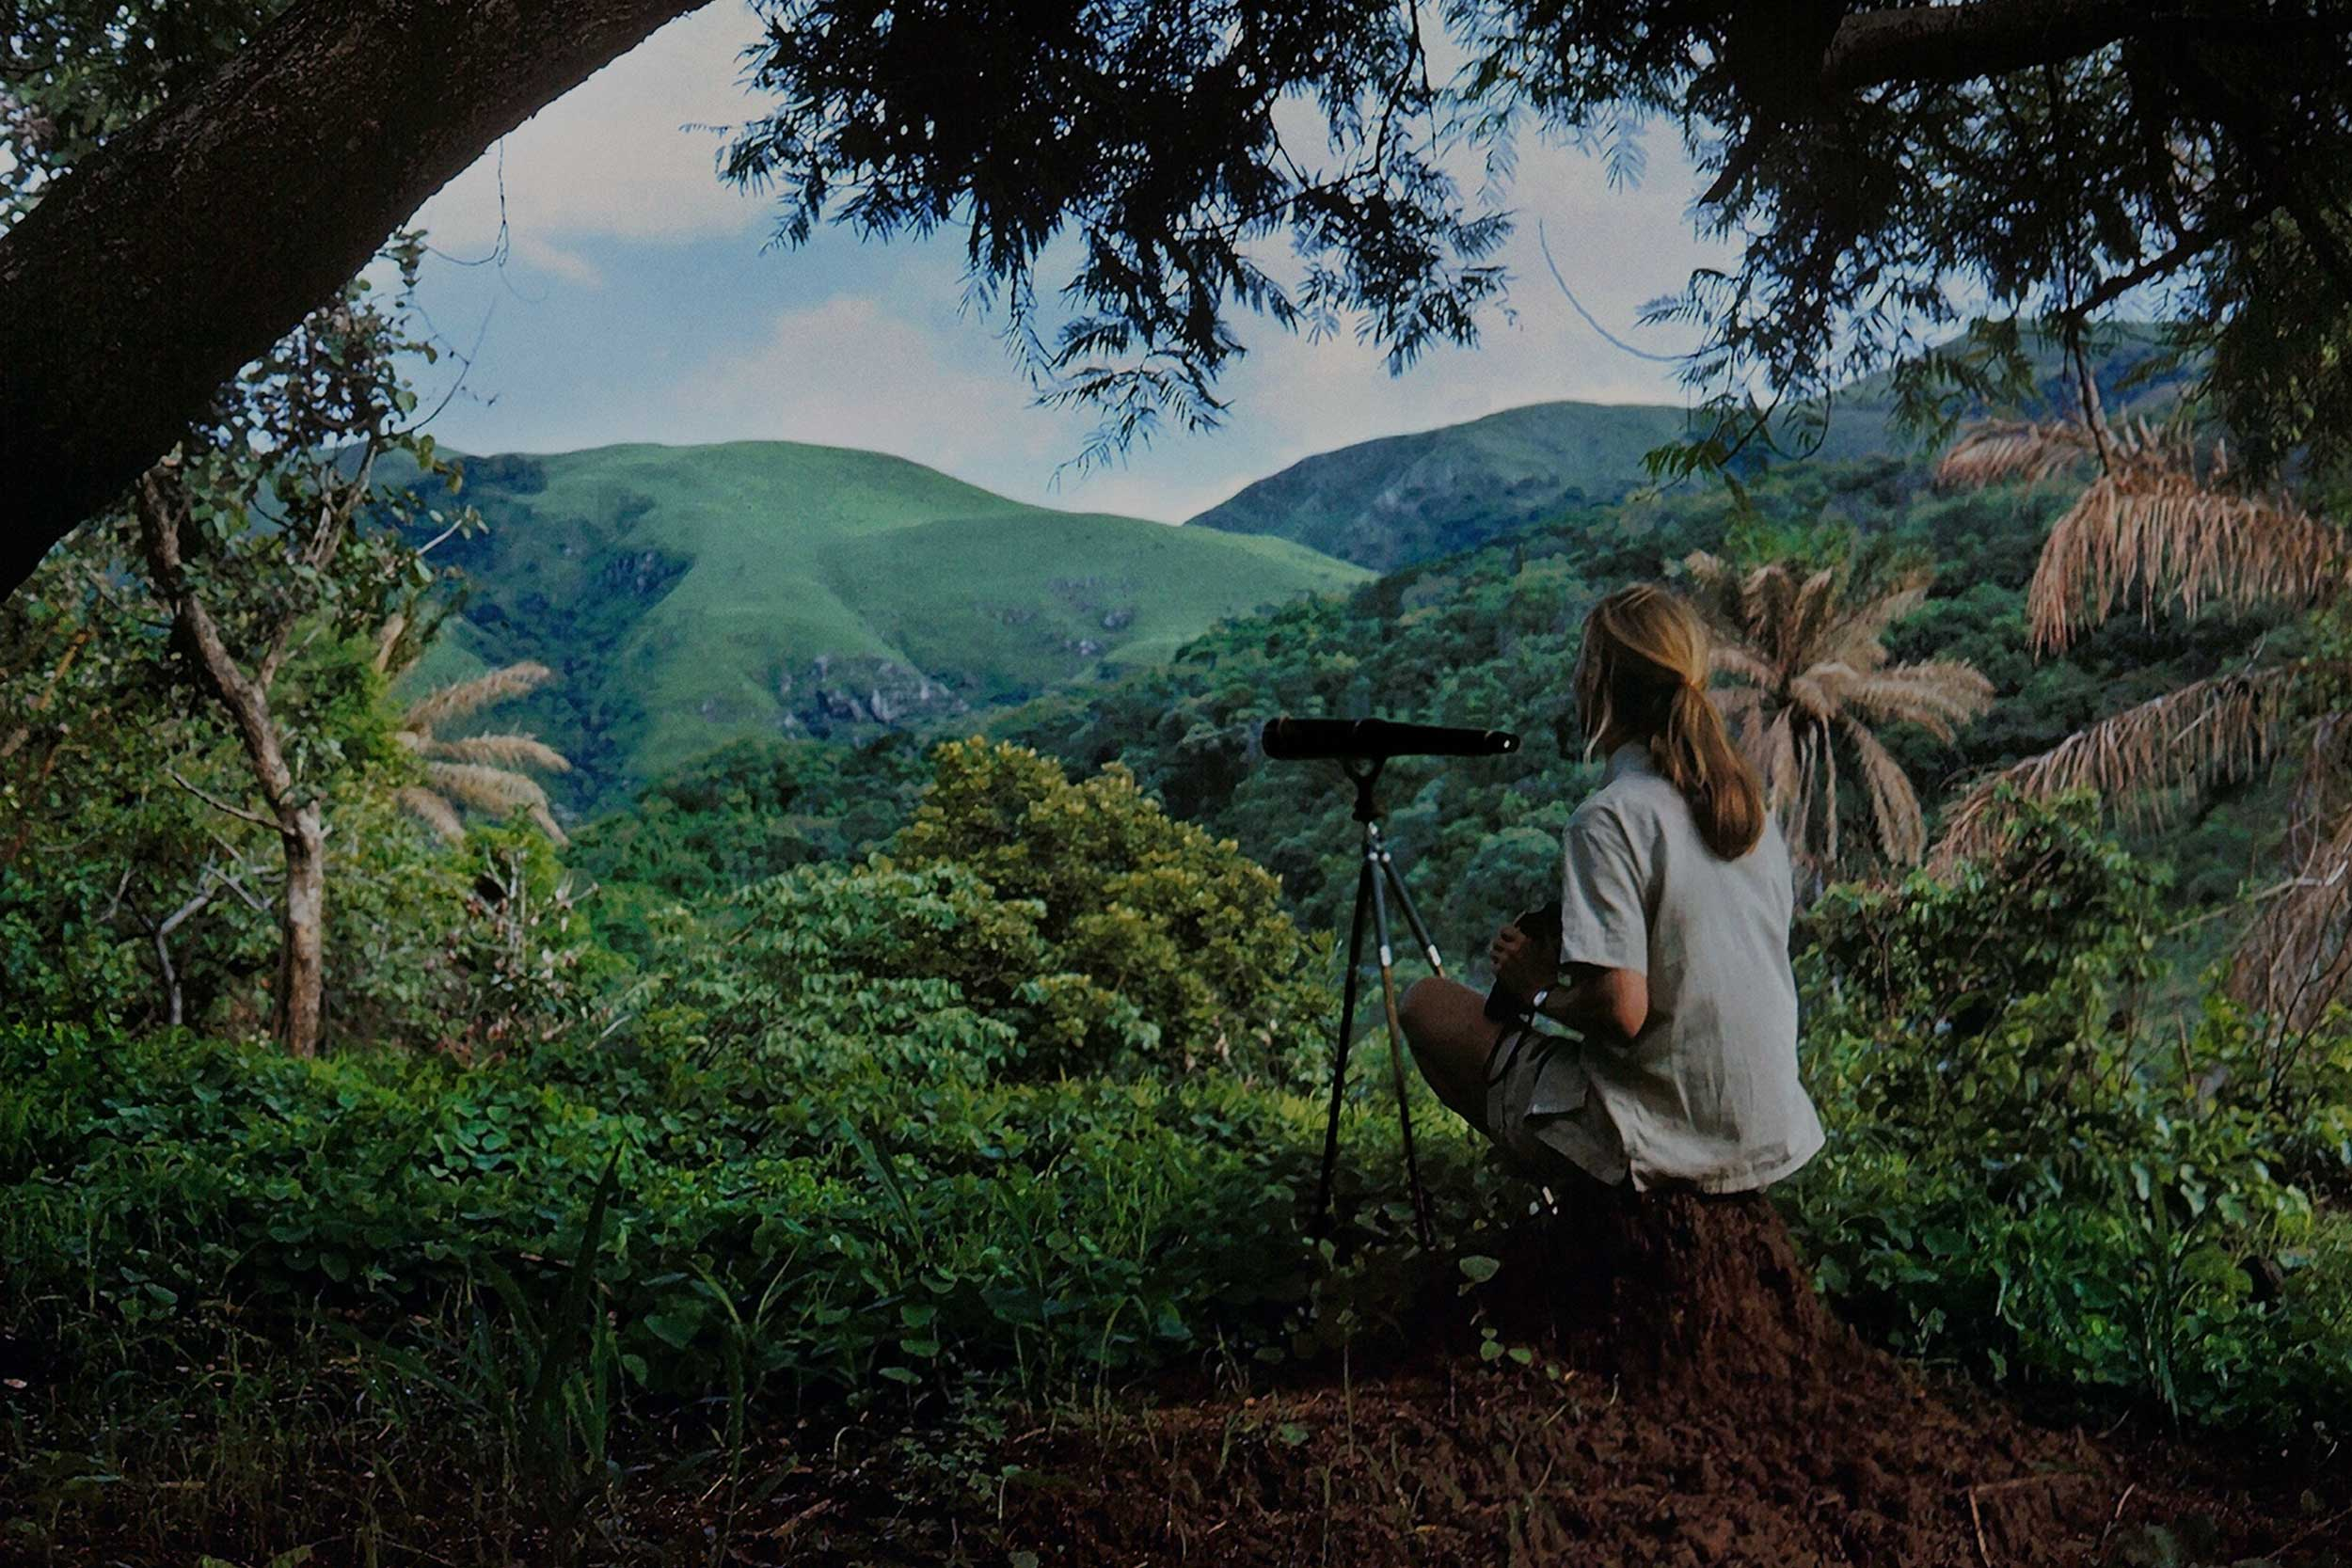
\includegraphics[
    width=8cm,
    height=8cm,
    keepaspectratio
]{jane-goodall-forest}

Goodall did this with the objective of helping us gain more insight into
chimpanzees and their relation with humans.

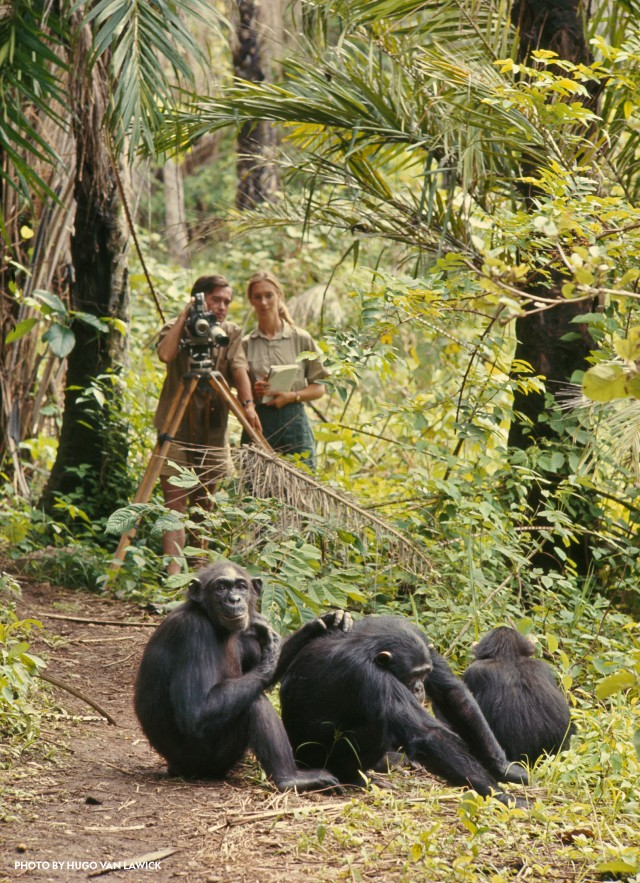
\includegraphics[
    width=10cm,
    height=10cm,
    keepaspectratio
]{jane-goodall-observing-2}

\pagebreak

And 5 years later, leading us to 1965, Jane Goodall finally earned her Ph.D.
from Cambridge University for her groundbreaking research on wild chimpanzees.

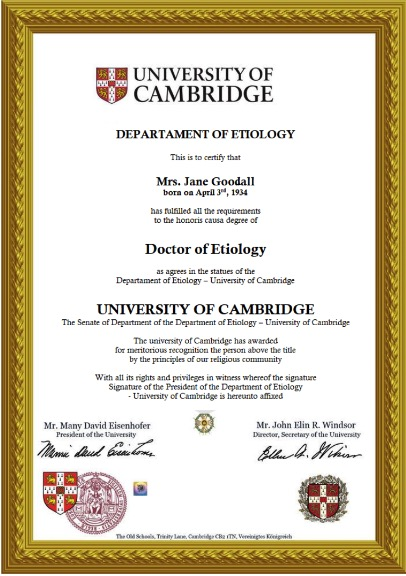
\includegraphics[
    width=10cm,
    height=10cm,
    keepaspectratio
]{jane-goodall-phd}

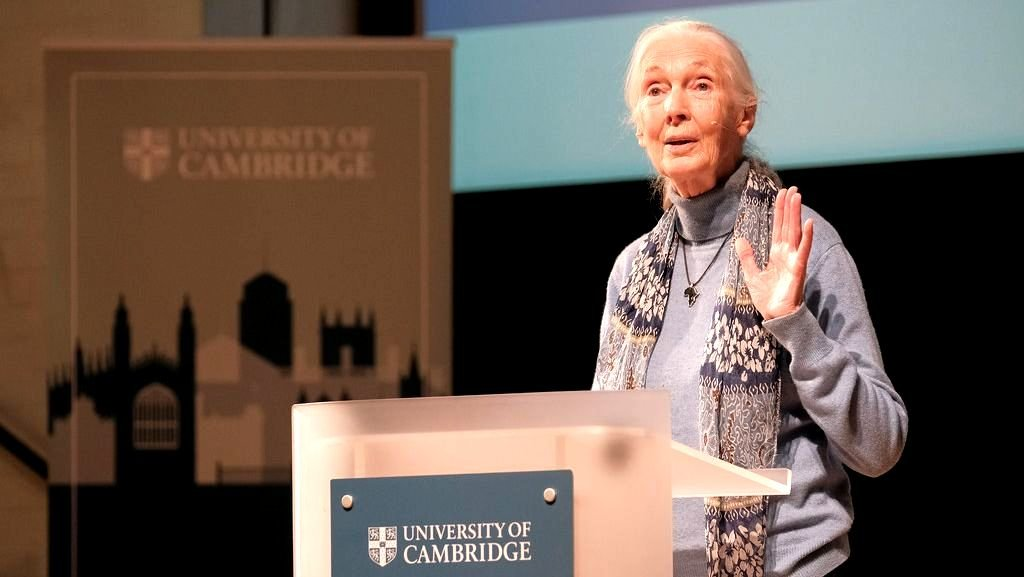
\includegraphics[
    width=11cm,
    height=11cm,
    keepaspectratio
]{jane-goodall-university-speech}

\pagebreak

\end{document}
